\documentclass[border=2pt, 10pt]{standalone}

\usepackage[dvipsnames]{xcolor}
    \definecolor{GDLcolor}{HTML}{A6A6A6}
    \definecolor{ELcolor}{HTML}{E8E490}

\usepackage{tikz}
    \usetikzlibrary{math}
\usepackage{siunitx}
\sisetup{%
    mode=math,
    per-mode=power,
}

\begin{document}
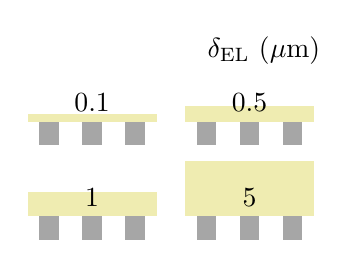
\begin{tikzpicture}

    \tikzset{%
        pics/deltaEL/.style args={#1/#2}{%
                code={%

                        \tikzmath{%
                            \dpore=0.3;
                            \epsilonGDL=0.55;
                            \deltawall=(1-\epsilonGDL)*\dpore/\epsilonGDL;
                            \deltafig=3*\dpore+3*\deltawall;
                            \deltaGDL=0.3;
                            \deltaEL=#1;
                        };

                        \fill [ELcolor, opacity=0.7] (0, 0) rectangle (\deltafig, \deltaEL);
                        \foreach \i in {0, ..., 2} {%
                                \fill [GDLcolor] ({\dpore/2+\i*(\deltawall+\dpore)}, 0) rectangle ++(\deltawall, -\deltaGDL);
                            }
                        \node at (\deltafig/2, 0) [above] {#2};

                    }
            }
    }

    \pic at (0, 0) {deltaEL=0.1/0.1};
    \pic at (2, 0) {deltaEL=0.2/0.5};
    \pic at (0, -1.2) {deltaEL=0.3/1};
    \pic at (2, -1.2) {deltaEL=0.7/5};
    \node at (3, 0.9) {$ \delta_{\mathrm{EL}}~(\mu\unit{\meter}) $};

\end{tikzpicture}
\end{document}